\documentclass[9pt,twocolumn,twoside]{osajnl}
\usepackage{xeCJK}
\usepackage{indentfirst}
\usepackage{niceframe}
	 \usepackage{listings}
	 \usepackage{xcolor}
	 \definecolor{mygreen}{rgb}{0,0.6,0}
	 \definecolor{mygray}{rgb}{0.5,0.5,0.5}
	 \definecolor{mymauve}{rgb}{0.58,0,0.82}
	 \lstset{
	 	backgroundcolor=\color{lightgray}, 
	 	%basicstyle = \footnotesize,  
	 	basicstyle=\ttfamily\footnotesize, 
	 	breakatwhitespace = false,        
	 	breaklines = true,           
	 	captionpos = b,                    
	 	commentstyle = \color{mygreen}\bfseries,
	 	extendedchars = false,             
	 	frame =shadowbox, 
	 	framerule=0.5pt,
	 	belowskip=-0.8 \baselineskip,
	 	keepspaces=true,
	 	keywordstyle=\color{blue}\bfseries, % keyword style
	 	language = C++,                     % the language of code
	 	otherkeywords={string}, 
	 	numbers=left, 
	 	numbersep=5pt,
	 	numberstyle=\tiny\color{mygray},
	 	rulecolor=\color{black},         
	 	showspaces=false,  
	 	showstringspaces=false, 
	 	showtabs=false,    
	 	stepnumber=1,         
	 	stringstyle=\color{mymauve},        % string literal style
	 	tabsize=2,          
	 	title=\lstname                      
	 }
\journal{ol} % Choose journal (ao, aop, josaa, josab, ol)

% See template introduction for guidance on setting shortarticle option
\setboolean{shortarticle}{false} 
% true = letter / tutorial 
% false = research / review article 
% (depending on journal).


\title{基于三维五子棋对弈的多人蒙特卡洛树搜索算法}

\author[1]{吴佳成}

\affil[1]{南开大学,软件学院,软件工程专业,三班,1412649}

%% To be edited by editor
\dates{\today}

\begin{abstract}

\ \ \ \ \ 基于蒙特卡洛树搜索(以下简称MCTS)来解决对弈问题的想法早已有之,然而MCTS算法在多人对弈中的研究并不常见。多人对弈在实际应用中,如果不加以任何的改进,就会遇到种种问题,从而导致该算法不能较为有效的应用在该情景中。而本文用一些相对较为简单的五子棋为例来进行多人对弈的蒙特卡洛树搜索。
\newline
\newline
关键字:多人对弈、蒙特卡洛树搜索
\end{abstract}

\begin{document}

\maketitle

\section{引言}

2016年,AlphaGo\cite{AlphaGo}一举在围棋上战胜了李世石,从而再一次引起了人工智能的一波春天。其中,主要用到的技术就包含了MCTS算法来作为增强学习,通过概率的方法达到以较小的代价来搜索尽可能多的情况,从而能够在游戏中表现出较为强悍的智能。然而,目前在大量的应用中,MCTS依然主要以双人对弈为主,似乎比较少用在多人对弈中。

在本文将该算法推广到多人对弈的情况时,的确,也遇到了种种障碍。一方面,多人对弈中的参与者之间的关系较为复杂,可以预见到参与者与参与者之间的关系并不只是像双方对弈之间的“零和博弈”——敌方损失等于己方获利,往往在多方对弈中可能会出现“合作”与“背叛”。另一方面,当引入了更多敌手的情况下,为了让机器的思考能够顾及到更多人的选择,所需要搜索的深度也应该有所增加,以防止出现过分“短视”的情况。

因此,为了更好的说明以上的情况,本文选择了一个具体的多人对弈的案例——三维五子棋,并针对以上提到的问题进行具体吻戏并尝试解决之。

\section{游戏规则说明}

如题目所说,该游戏为三维情形的五子棋游戏,只要在各种方向上能够连成五个即可,其中方向共包含13个方向,分别为沿轴方向($x,y,z$)共三个,面对角线方向($x^+y^+,x^+y^-,y^+z^+,y^+z^-,z^+x^+,z^+x^-$)共六个方向,以及体对角线方向($x^+y^+z^+,x^+y^+z^-,x^+y^-z^+,x^+y^-z^-$)共四个方向。棋盘格为6*6*6,共计216种落子情况。

这边需要特别说明的是,本来平面五子棋的游戏适合两人进行对弈,而并不适合多人对弈,因为其可以连成五子的方向共计只有四种可能,所以多人玩的话,失去了娱乐性。而推广到三维的时候,可以看到可以连成的方向变得非常多,即自由度提升了,如果此时依然还是两人对弈,那么先手就具有更大的优势——进行堵截的难度大于连子的难度。所以,将这个游戏相对更加适合三人以上进行对弈。三人进行对弈的话能够较好的平衡自由度过大带来的问题。

\section{问题}

使用MCTS算法使得三台机器在三维五子棋游戏上进行“合理的”对弈,并能够较好的解决上述遇到的推广中存在的困难。

\section{基本的MCTS}

本章节简单的介绍一下MCTS\cite{MCTS}。MCTS主要分为四部分:选择(Selection),扩展(Expansion),模拟(Simulation),回传(Backprogation)。

\begin{figure}[htbp]
	\centering
	\fbox{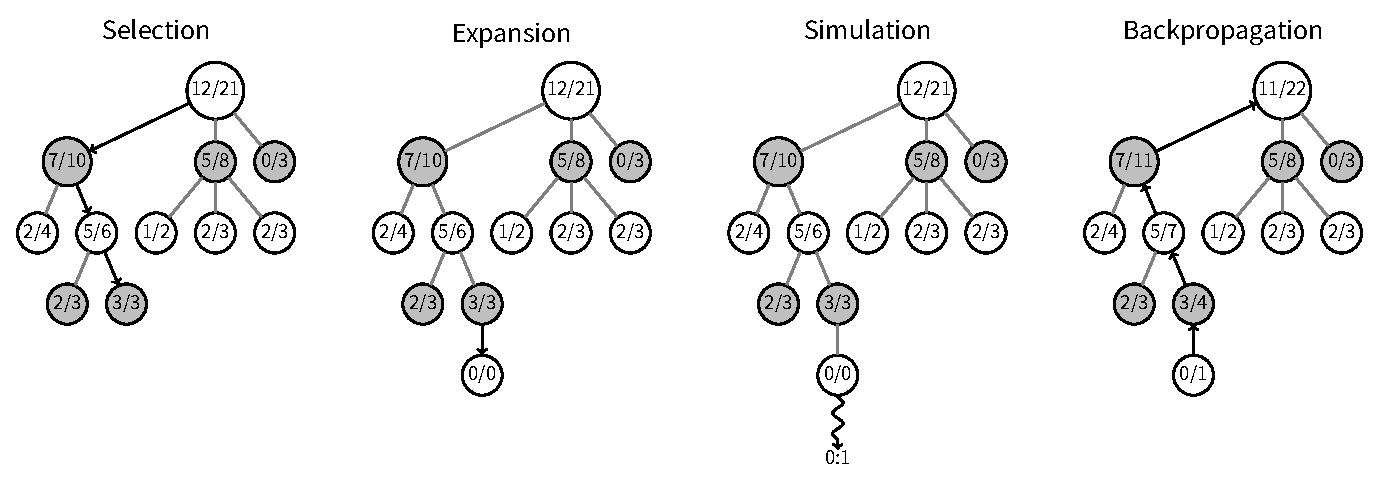
\includegraphics[width=\linewidth]{MCTS.eps}}
	\caption{关于MCTS的流程 \ 来源WIKI \cite{MCTSGraphWiki}}
	\label{fig:false-color}
\end{figure}

上图较好的阐述了MCTS的算法主要流程。

以下对四部分进行更为详细的阐述:
\begin{enumerate}
	\item 选择,通过一些策略(主要进行改善的部分)对已经掌握的模拟数据来判定敌方和己方下一步最有可能选择的步骤,一直到叶节点(没有模拟数据的节点)
	\item 扩展,在已经达到的叶节点,选择其可能的下一步骤,生成叶节点加入到搜索树中,一般而言,会进行随机选择节点(为了效率,然而也可以使用其他的一些策略来进行,比如使用卷积神经网络进行评估)
	\item 模拟,当选择好需要扩展的节点之后,就以随机的方式来进行模拟接下来的步骤,直到游戏终止,此时或者抉择出输赢,或者平局。
	\item 回传,根据模拟的局势进行评估,并将得到的记录从扩展后的叶节点传递到根节点。
\end{enumerate}
然后以上过程会迭代到指定的次数,本文代码中一般指定1000000次左右。
可以发现通过迭代会有越来越多的节点加入,同时最开始加入的节点(一般也是上层的节点,代表离当前状态较近的状态以及落子)也获得了较多模拟,从而在概率上能够逼近该落子之后真正获胜的概率。

之后简要介绍一下MCTS算法如何应用在棋局上。具体方法如下:每一次需要决定下一着落子在何处时,将当前状态作为根节点,开始进行MCTS的迭代,迭代到指定次数后,当前状态对应的根节点的直接孩子节点所对应的状态就是下一着所有可能落子之后的状态。因此根据其直接孩子节点的模拟状态结果来进行选择下一个状态,从而选择出对应的落子。

伪代码如下:
\begin{algorithm}
	\caption{MCTS algorithm}\label{alg:MCTS}
	\begin{algorithmic}[1]
		\Procedure{ComputeMove}{$rootState$}
		\State $rootNode = create \ from \ rootState $
		\While{$up \ to \ max \ iterations$}
		\State $node = rootNode$
		\State $state = rootState$
		\While{$node \ != NULL || node \ tried \ all \ moves$ }
		\State $node = select \ child \ from \ node \ by \ policy$
		\State $apply(state,node.move)$ \Comment{selection}
		\EndWhile
		\State $select \ random \ feasible \ move$
		\State $apply(state,move)$
		\State $newNode = create node from state$
		\State $node.add\_child(newNode)$ \Comment{expansion}
		\While {$state \ is \ end$}
		\State $apply(state, randon \ move)$ \Comment{simulation}
		\EndWhile
		\State $result = get\_result(state)$
		\While {$node == null$}
		\State $node.update(result)$\Comment{back prop}
		\EndWhile
		\EndWhile
		\State $get \ specific \ child \ from \ rootNode$
		\State $get \ according \ move$
		\State $\textbf{return} move$
		\EndProcedure
	\end{algorithmic}
\end{algorithm}

\section{扩展多人对弈的问题}
在引言中,已经提到了关于使用MCTS来解决多人对弈的问题。现在来详细的阐述。
\subsection{$\cdot$ 合作与对抗}
\begin{adjustwidth}{2em}{}
	\ \ \ \ \
	
	三人游戏中,并不简单的存在着对抗的状态,而是可能会存在短暂的合作的情况,为了更好的理解这个情况,下面以一个例子来进行说明
	
	\begin{figure}[htbp]
		\centering
		\fbox{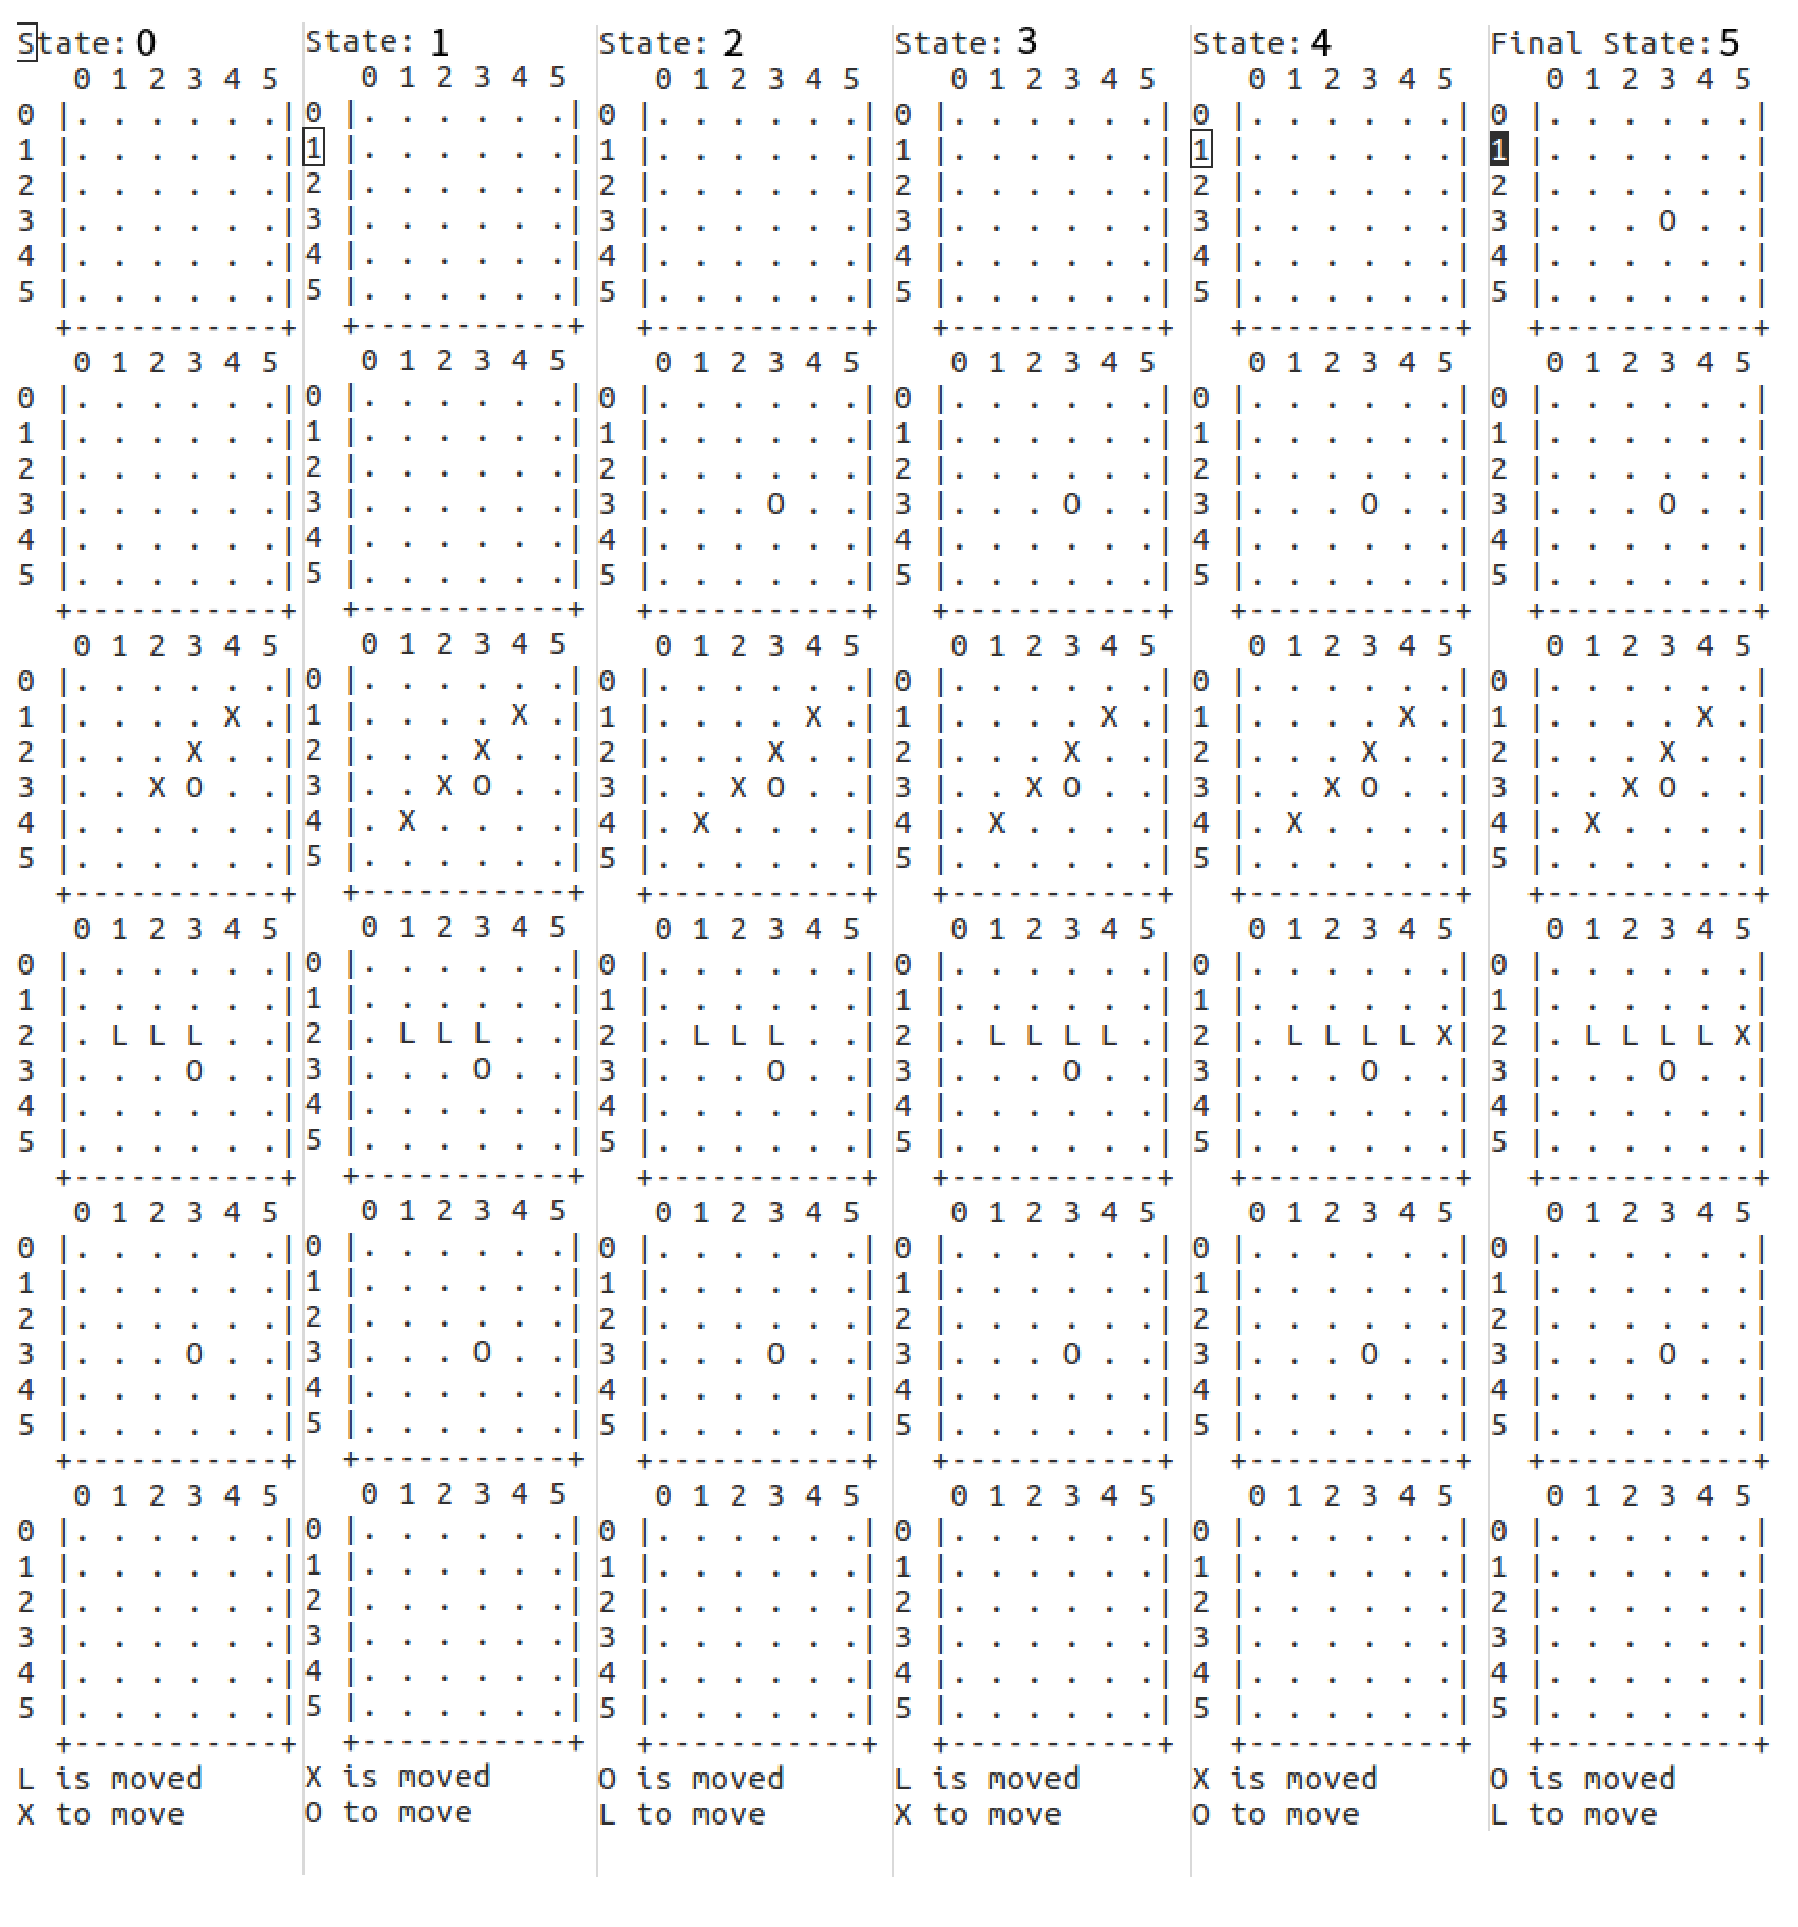
\includegraphics[width=\linewidth]{failureCase.eps}}
		\caption{原始MCTS形成的局面,迭代次数1000000}
		\label{FailureCaseStudy}
	\end{figure}	
	

	
	见图\ref{FailureCaseStudy},具体遇到的问题是这样的。其中下棋初始顺序为X,O,L。起初,大家各自尽量连成线,并纷纷占据中间有利位置。然而当遇到了状态0的情况,即X首先连成三个子,而O需要进行做选择的时候。
	
	如果MCTS不加以改变就直接运用在多人游戏上,就会出现这样的情况。是的,种种原因,导致了该局面的发展变得似乎有些“弱智”,是的,大家都光顾着自己要连成子,却并没有去堵别人,从而导致先手必胜的结果。
	
		\begin{figure}[htbp]
			\centering
			\fbox{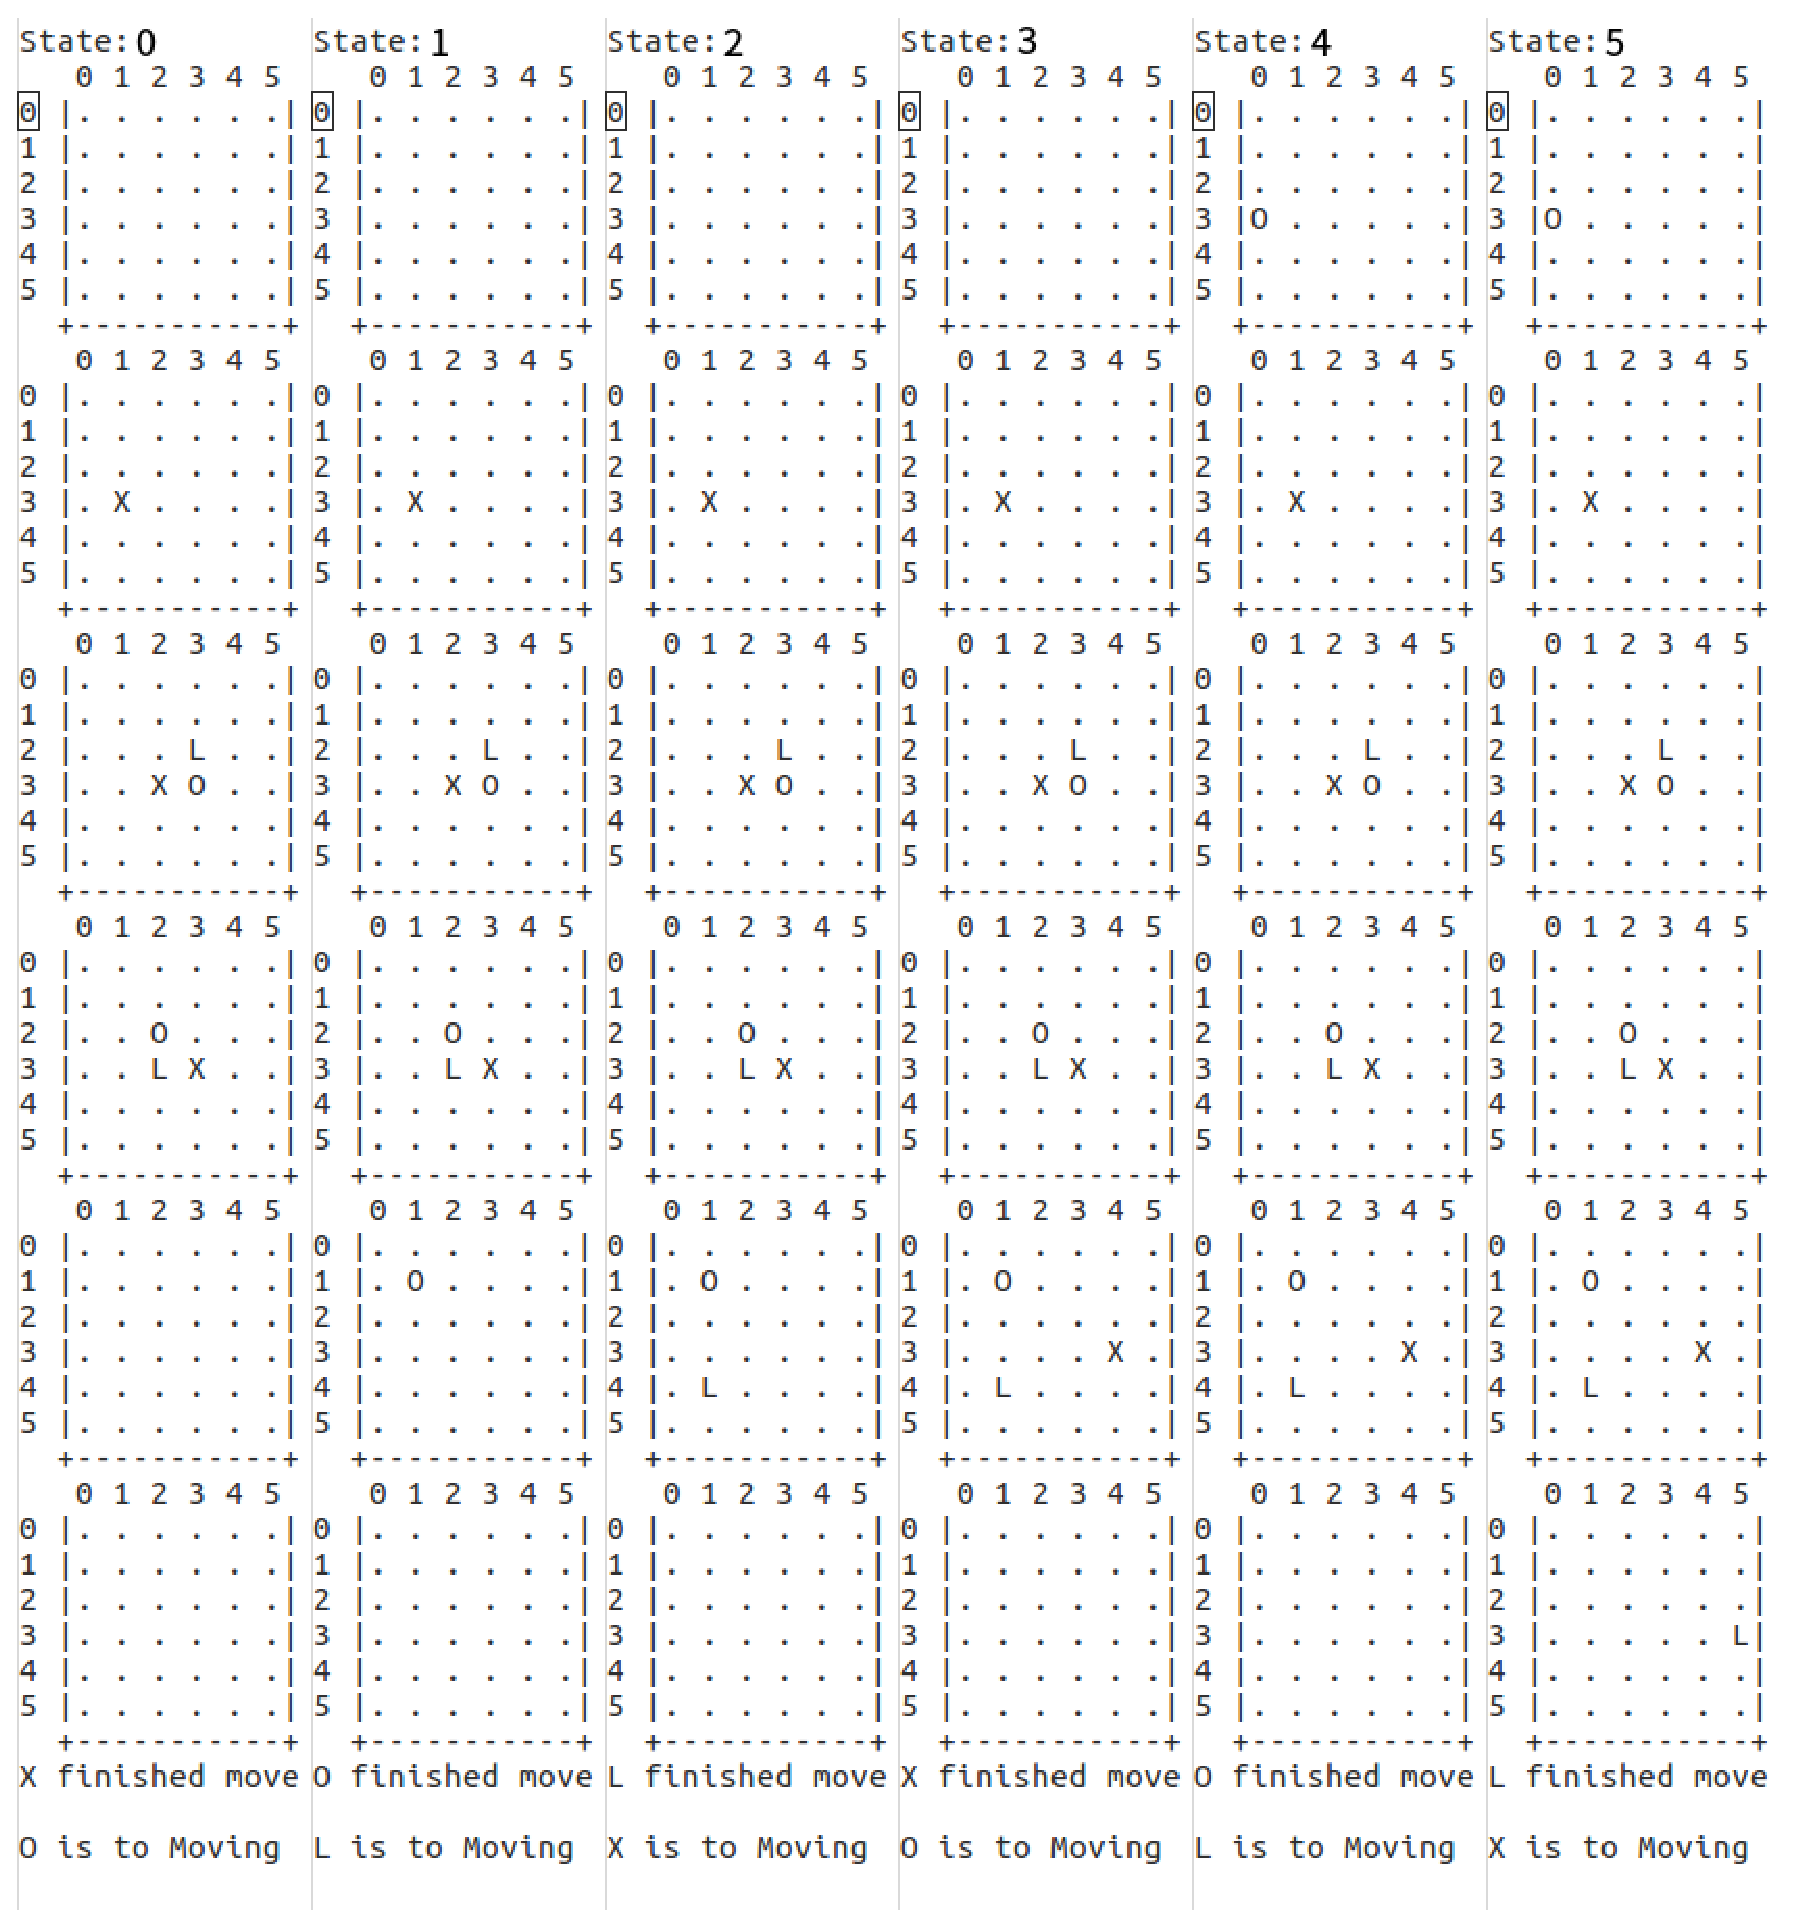
\includegraphics[width=\linewidth]{state.eps}}
			\caption{比较合理的局面,迭代次数1000000}
			\label{caseStudy}
		\end{figure}
	
	一般而言,如果是双人五子棋,那很自然的就应该是去选择封住对手,否则四个子连成线还没有来赌的话,几乎是必输的。然而在这里就不一样了,比较合理的做法应该如图\ref{caseStudy}。就是O和L也应该分别先扩展自己的连子(State 1, State 2),一方面增大自己连成子的数目,另外一方面也让自己占据的棋盘的自由空间较多。接下来X继续下第四招形成四连子(State 3)。这时候剩下的两方应该合力将其围堵(State 4, State 5)。可以说,这样的选择是明智、合理且最优的。
	
	当然在这更之前进行堵截也是合理的。
	
	因此可以发现,在合理的多人游戏中,的确会出现短暂的结盟,从而达到自己的最优化,可以看出,因为短暂的结盟的产生,L和O都在状态结束后获得了三连子。
	
	不过,如果继续研究的话,会立刻发现这个联盟立刻就要瓦解,同时会建立新的结盟。因为X目前是不能导致新的危机,而此时X必然会选择扩展自己的领域,再下一步就会产生新的O四联子,从而会再次导致L和X结盟。从而棋局会发展的比较复杂。
	
	
	综上,可以发现三人游戏在战略上复杂程度和二人对弈完全不一样。
	
\end{adjustwidth}
\subsection{$\cdot$ 要求搜索深度、广度的增加}

\begin{adjustwidth}{2em}{}
	\ \ \ \ \
	为什么会形成这样的弱智原因呢?这边也做一下简单的分析。因为当参与者变多的时候,如果需要考虑到自己的下两步骤的话,需要考虑剩下其他人所有的下一步应该如何落子,而有由于状态爆炸,可以明显的发现就连三人参与游戏的时候,所需要搜索的空间就应该达到原来二人对弈的200多倍才能达到所希望的智能程度,这个是难以接受的。
	
	依然还是用之前的场景(图\ref{FailureCaseStudy})来说明这个情况。显然,基于MCTS的逻辑,在状态3的时候,O主动去探寻下一步大约有200种可能,都进行尝试,但是此时的输赢实际上关系到L的选择,因此有需要200种可能,然后之后又取决于X的选择,有存在200种可能,等探索到正确的分支已经需要200*200*200个情况,而总共迭代次数设置1000000,可能还没等探索到合适的分支就结束了,或者就是概率上探索到了该分支,也没有多少试验落到该分支。同时由于概率性的原因,还有可能X不选择必胜步骤,所以还会继续实验下去种种原因。都导致了O并不会去选择拦截X的行动,从而发生了这样的情况。
	
\end{adjustwidth}

以上问题使得传统的MCTS在该游戏中(多人游戏)遇到了困难,当然疯狂的增加迭代次数固然是一种方案,然而所需要的代价太大,以下本文就提出一些方案来尝试解决。

\section{对MCTS的改变}
基于以上问题,本文对MCTS进行了一些改变,阐述如下:
\subsection{$\cdot$ 状态向量化反传\cite{MCTSMPG}}
\begin{adjustwidth}{2em}{}
	\ \ \ \ \
该思路来源于\cite{MCTSMPG}提到的内容,简单来说,就是原来的MCTS只是将输赢反传回去,这在二人博弈中,没有问题,A赢就是B输,反之亦然。不过多人中,A输并不代表B赢,还有可能是C赢。因此为了能够更好的跟踪当前局势以及后续分析,我们应该同时记录其他所有人的状态。

所以本文在Simulation结束后,将获得的结果打包成一组向量$(x_1,x_2,x_3)$,用于反传的过程。而每一个节点收到这个向量之后,也分别对自己保存的向量的每一维进行更新。
\end{adjustwidth}
\subsection{$\cdot$ Selection的Policy改变}
\begin{adjustwidth}{2em}{}
\ \ \ \ \ 原本的MCTS的policy的公式为$\dfrac{w_i}{v_i}+C\cdot\sqrt{\dfrac{\ln{\sum_{i}v_i}}{v_i}}$。其中,$w_i$为第i个节点的获胜的次数,每次获胜记为1,平局0.5,输为0,$v_i$为第i个节点访问次数。因此,在二人对弈的时候,上面公式的两部分很好的均衡了收益与探索之间的均衡。

然而,在多人对弈中,上面的式子则相对有所欠缺。主要基于以上问题的考虑——缺乏合作与竞争。

因为在三人游戏中(多人游戏同理),\textbf{增大自己的获胜概率和减小他人的获胜概率并不完全等价}(注意:这和二人博弈有较大的区别)。以下举例说明:

\

\fbox{\begin{minipage}{22em}
		在四人局中,A,B,C,D按顺序落子,此时A已有四个子连在一起,且两边没有阻挡,而B现在也已经有三连子。现在轮到B做决策,如果B想要增大自己的获胜概率,那么应该让自己的三连子变成四连子;如果B要减少他人的获胜概率,那么应该去阻挡A的四连子。
	\end{minipage}}


\ \\


通过以上例子,就可以知道在三人中两种情况的区别。那自然为了解决这个问题,可以对Policy公式进行修正。本文对该公式新添加一项——抑制对手项,简单来说,就是让最大非本人可能获胜的概率尽可能小,单项公式如下:

\

\fbox{\begin{minipage}{22em}

$\max\limits_i(1-\dfrac{\max\limits_{j\neq k}{w_{ij}}}{v_i})$

$k$为参与人的标志

$w_{ij}$代表了$i$节点的参与人$j$获胜的状态

$v_i$代表$i$总共被访问的次数。
	\end{minipage}}

\ \\

因此,将这个公式与原始的Policy何在一起,就有如下公式(符号已在上述公式中解释):

$\mathop{argmax}\limits_i(A\cdot \dfrac{w_{ik}}{v_i}+B\cdot(1-\dfrac{\max\limits_{j\neq k}w_{ij}}{v_i})+C\cdot\sqrt{\dfrac{\ln{\sum_{i}v_i}}{v_i}})$

本文通过以上策略进行Selection步骤,较好的考虑了三者之间的关系,能够解决MCTS原本在多人对弈中遇到的问题。

同时,需要说明的是,可以通过调整三者前面的参数,可以让参与人表现出不同的策略,是更倾向于冒险,还是更倾向于保守。

这边,还有一个需要注意的地方,这边选择相同的策略对每一步(包括对手的落子)基于这么一个前提假设:\textbf{如果某人的思想是激进的,那么该人也会认为对手也是激进的,反之亦然},尽管实际上可能并不如此,但是这个假设还是在很大程度上符合真实的情况,并且在实际上也并没有引起问题。另外,尽管可以引入策略的组合,即某人认为自己是激进的同时,认为敌方采用保守策略,然而这样引入过多的参数就有一些过拟合的倾向,因此不予亦采用。
\end{adjustwidth}

\subsection{$\cdot$添加合理的剪枝策略}
\begin{adjustwidth}{2em}{}	
	\ \ \ \ \
	该章节对剪枝策略进行描述,实际上MCTS本身是不包含任何剪枝过程,因为如果能够有足够多的迭代次数,一些不合理的分支的评分会非常小,从而顺利被减掉。然而在本游戏中,总共有$216!$这么多种可能性,单纯依赖MCTS的“自助剪枝”显然是不科学的,并且该情况也在实践中证明这一点。

	而对那些较为上层的节点的剪枝过程具有较大的不确定性,可能会减去一些应该选择的情况,从而导致失败。因此为了在合理和效果上的权衡,我们应该尽可能选择靠近终局的状态进行剪枝。
	
	同时需要注意的是,任何剪枝过程都发生在迭代中,所以也是时间开销较大的部分,如果每一次剪枝都耗费大量时间,那样也会极大的增大时间开销,从而只能够缩减模拟的次数。这是得不偿失的。因此,剪枝策略一定要快、准。
	
	因此本文在此处采用了一些模拟过程策略:
	\begin{enumerate}
		\item 当在开始模拟前,状态就已经达到终局,并且分出胜负,那么需要将该父亲节点的其他所有选择可能都减去。同时立刻修改父亲节点的胜率。
		
		该策略基于以下考虑:如果开始模拟前达到终局,只能说明扩张的这一步就是在之前状态的某一方的必胜步骤,因此不论如何,在模拟过程中都应该假设这一步无论是哪一方一定会选择的一步。
		
		\item 当开始模拟的第一步之后,就遇到了游戏终局,并且已经分出胜负,那么此时应该将这一步选择对应的节点加入到模拟开始前的节点A,并将A节点的其他分支和可能移动步骤删除,同时修改胜负率。
		
		修改胜负率的逻辑如下:获取下一步的移动者,将该移动者对应的胜率置为1,其他置为0。
	\end{enumerate}
	
	以下的图示对以上策略进行说明,为了简便期间,只用二人对弈来说明,可以简便的推广到多人对弈。
	
	\begin{figure}[htbp]
		\centering
		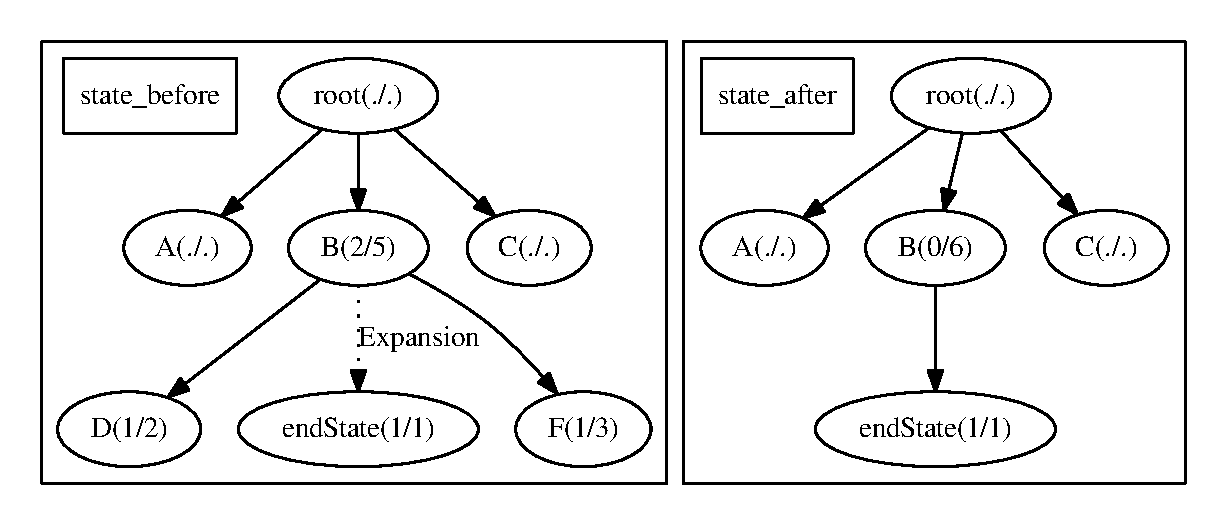
\includegraphics[width=\linewidth]{policy1.eps}
		\caption{剪枝策略1说明}
		\label{fig:policy1}
	\end{figure}
	\begin{figure}[htbp]
		\centering
		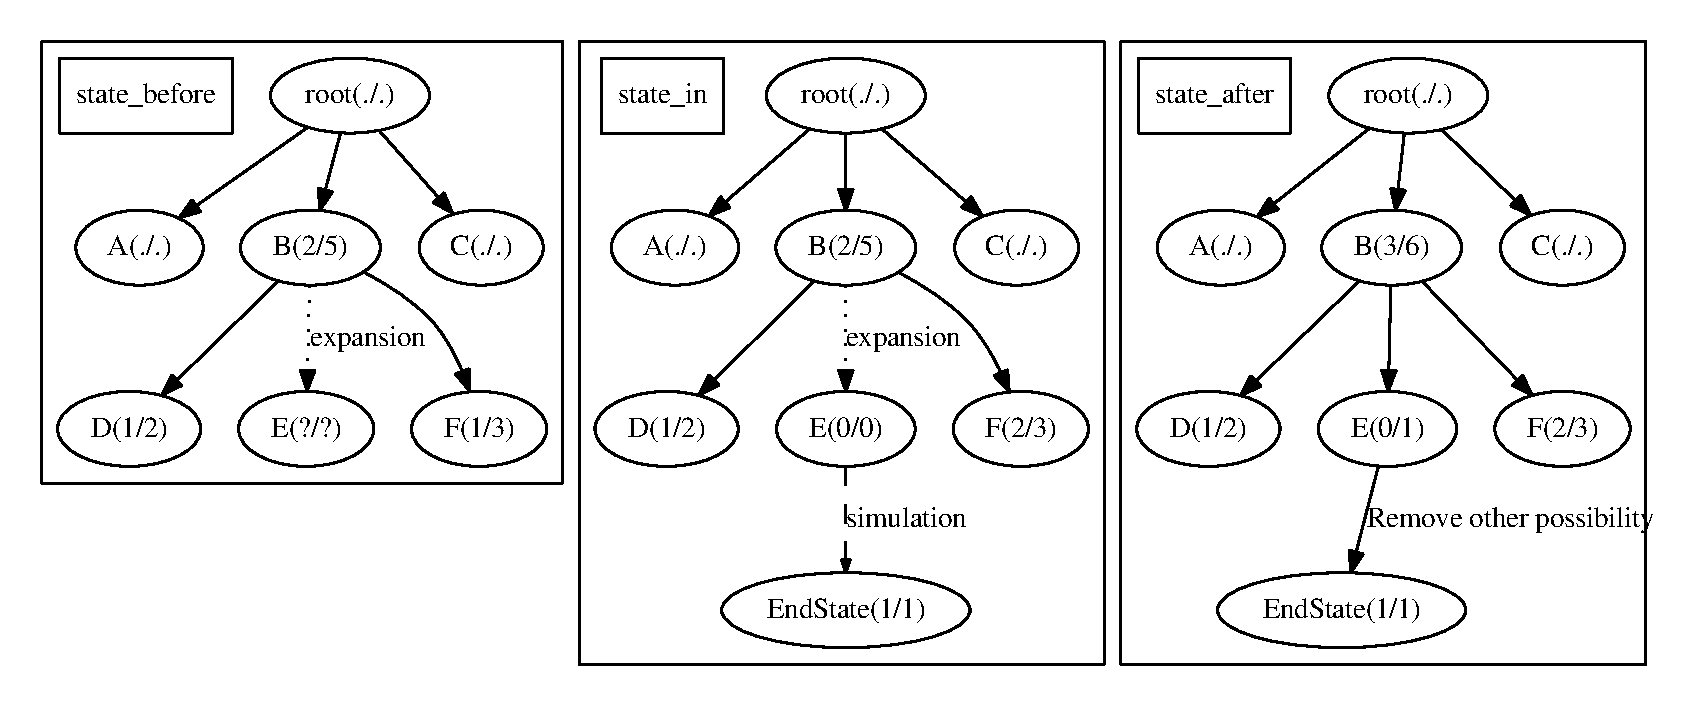
\includegraphics[width=\linewidth]{policy2.eps}
		\caption{剪枝策略2说明}
		\label{fig:policy2}
	\end{figure}
	
	可以发现,以上两个步骤都是基于这样的逻辑:\textbf{当下一步会取得胜利的时候,有理由相信,无论是对方还是己方,一定会选择这一步}。可以说这个假设非常的朴素,但是非常有效,这也说明了一点:在增强学习中,假设对方更加聪明的同时,也让自己变得更加聪明。
	
	不过以上的剪枝逻辑个人看来,并不容易继续扩展,因为该逻辑的主要能够直接影响已经建立起来的树的节点,然后当一次模拟的次数超过2次之后,其最终状态对应的节点和父亲节点都没有在已有的搜索树建立起来,更谈不上剪枝的说法。
	
	
	
\end{adjustwidth}
\subsection{$\cdot$合并迭代的搜索树}
\begin{adjustwidth}{2em}{}	
	\ \ \ \ \
	在MCTS中,每一次需要计算新的落子的时候,都会基于当前状态重新建立一个新的生成树,然后进行MCTS的迭代。
	
	然而,实际上,每一次搜索树结束之后,直接丢弃有一些可惜,所以本文的想法就是自游戏开始知道结束都维护着一棵树。具体步骤如下:
	
	\begin{enumerate}
		\item 第一次进行预测前,创建一个空树
		\item 进行预测的时候,在该树上进行改进后的MCTS算法
		\item 当真正的游戏中选择了具体的一步,选择该树对应步骤的子节点,成为新的根节点。
		\item 接下来,每一次进行预测都使用该根节点,直到游戏结束。
	\end{enumerate}
	
	以上就是将搜索树进行合并的思路,代码层面也非常方便实现,并且能够较好的利用之前的获取的成果。
	
	这边,需要说明的是,合并是否是合理的。这个合并实际上在某种意义来说,是不合理的,因为A参与者理论上来说不应该基于B参与者MCTS算法之后的树。
	
	但是可以用以下的逻辑来解决这个问题,在B参与者进行MCTS的算法时,A参与者也可以同时进行对B的下一招进行预测的MCTS算法。这个逻辑是合理的,因为两者的思考是独立的,然后我们可以将合并搜索树看做是这个情况的一种近似模拟,同时还能节省计算时间,否则每一个时刻都需要同时模拟三人的MCTS。
	
\end{adjustwidth}

\subsection{$\cdot$三种方法共同运用时的分析}
\begin{adjustwidth}{2em}{}	
	\begin{enumerate}
		\item \textbf{剪枝和合并}
		 
		 \ \ \ \ \ 其实合并规则运用在原来的MCTS上本身是没有意义的,因为对于给定一个状态,其后续选择是200种可能,因此分摊到具体的一种可能的迭代次数只有1/200这么多,这个对下一次模拟的影响几乎可以忽略不计。
		 
		\ \ \ \ \ 然而因为改进后的MCTS有了剪枝,而能够进行剪枝的节点不仅仅只出现在根节点的直接孩子节点,因此通过合并能够将剪枝的状态保存下来,从而能够更好的知道后续的搜索历程。
		\item \textbf{改进策略与合并}
		
		\ \ \ \ \ 其实多种策略与合并在某种意义上是有所冲突的,因为同一个树每一个节点的胜负率会随着不同的选择策略在概率意义上是不一样的,所以搜索树合并的时候在理论上来说上一次依据A策略进行的MCTS算法会干扰到下一次依据B策略的MCTS,这样是不合理的。
		
		\ \ \ \ \ 不过,实际上在这里,也不需要担心,因为和上面的逻辑一致,其实合并的重点并不是多模拟几次,相反,当局势推进后(根节点被新节点替代掉后),之前模拟的影响反而无足轻重。因此并不会干扰到下一次的模拟,所以合并在这个意义上是合理的。
		
	\end{enumerate}
	
	
\end{adjustwidth}
\section{失败的改进尝试}
尽管是一些失败的尝试,但是以下这些失败的尝试还是给我带来了很多的启发,所以这里还是进行了说明。
\subsection{$\cdot$按照随机次数来衰减模拟结果}
\begin{adjustwidth}{2em}{}	
	\ \ \ \ \
	这个本来是一个很自然的想法。因为在从一个扩展节点开始,进行模拟直到结束,会经过的步骤数量有多有少。因此这个数量也可以纳入考虑范围内。并且因为随机的次数越多,其获得的终局带来的结果越不可信,所以占据的比例应该更小。
	
	当模拟游戏达到终局后,获得了状态向量$(x_1,x_2,x_3)$,然后同时获得了模拟的次数$\phi$,然后获得新的状态向量$(x_1\cdot C^\phi, x_2\cdot C^\phi , x_3 \cdot C^\phi), 0<C<1$,将该新状态向量进行反传。
	
	然而实际上这个策略非但没有改善效果,相反让程序变得更加“弱智”了。
	
	实际上,后来分析了一下原因,这个是有原因的,因为在模拟过程中,每一次都是随机的,然而在一些“危急”的时刻,其实双方应该选择的步骤很少,但是由于随机性,很有可能会误认为对方会选择剩余的步骤,从而在很少的步骤内就结束了棋局。这种情况下,并不是下棋随机的次数越少越好。而且类似的情况在概率上来说并不是少见的情况。
	
	综上,使用随机次数进行衰减模拟结果是不合理的。
	
\end{adjustwidth}
\subsection{$\cdot$非确定性剪枝}
\begin{adjustwidth}{2em}{}	
	\ \ \ \ \
		在剪枝中,提到了这样的逻辑:\textbf{当下一步会取得胜利的时候,有理由相信,无论是对方还是己方,一定会选择这一步},并说明比较困难推广。本文也做了如下的尝试,但是效果都不尽人意。(然而也并不清楚为什么,可能是实现问题,或者迭代次数过少)
		
		如果尝试推广这样的逻辑,\textbf{如果下一步赢的概率很大的时候,有理由相信双方几乎一定会选择这一步}。
		
		所以在迭代过足够多次数之后,比如达到指定次数的一半以上,就会开启非确定剪枝,策略依旧比较简单:对于某一个节点,如果其某一个孩子节点的胜率还达不到所有孩子节点最高胜率的1/3(可以指定),可以认为该孩子节点几乎没有获胜的概率,并且不会被选择,从而减去该分支,以上操作会递归运行。
		
		然而,效果并不是很好,猜测应该是在递归运行的时候减去了本来应该能够获胜的分支。
\end{adjustwidth}

\section{实验}

\subsection{$\cdot$具体实现}
\begin{adjustwidth}{2em}{}	
	\ \ \ \ \
	代码主要以C++为主。
	
	主要代码改编于\cite{MCTSbasecode}。该代码实现了最原始版本的MCTS算法,其应用主要为双人博弈版本的connect\_four(落子只能在一维方向)的一个游戏。
	
	本文对该代码进行了修改,讲原本的代码该成了所需要的游戏逻辑,讲原本的二人对弈改成可以任意多人对弈的情形。同时将上述提到的各种思想全部加入到代码中,从而能够较好的模拟实际情况。
	
	值得说明的是,源代码为了能够加速运行,采用了多线程,本文的代码自然也采用了多线程,但是为了防止纠结在数据的一致性上,对于搜索树合并的行为指建立在同一个线程内,也即每轮迭代时相同编号的线程共享一个搜索树,并进行搜索树的合并。
	
	然后,本次代码也利用了C++模板的各种技巧,为了能够加速程序的运行,使用模板元编程技巧将各种可以编译期间常量化的数据都常量化,从而使得减少各种计算。同时也是为了更好的兼容性。
	
	这边对一些个人精彩的代码进行展示:

	 
\begin{lstlisting}
template<typename State, typename = void>
struct getSupportNumPlayers
{
	static const int value = 2;
};
	   
template<typename State>
struct getSupportNumPlayers<State, decltype(typename std::enable_if<std::is_integral<decltype(State::Support_Num_Players)>::value>::type())>
{
	static const int value = State::Support_Num_Players;
};
\end{lstlisting}
以上部分代码主要在编译期间确定一个具体的模板类是否包含具体的数据成员名字,如果包含并且是指定类型的话,就使用该数据成员对应的数值,否则选取默认值。

\begin{lstlisting}
namespace CONST_STATIC_ARRAY_GENERATOR
{
	template<char ... args> struct ArrayHolder { static const char data[sizeof ... (args)]; };

	template<char ... args>
	const char ArrayHolder<args ...>::data[sizeof ... (args)] ={ args ... };

	template<size_t N, template<size_t> class F, char ... args>
	struct generate_array_impl { typedef typename generate_array_impl<N-1,F,F<N>::value,args...>::result result; };

	template<template<size_t> class F, char ... args>
	struct generate_array_impl<0, F, args ...> { typedef ArrayHolder<F<0>::value, args...> result; };

	template<size_t N, template<size_t> class F>
	struct generate_array { typedef typename generate_array_impl<N-1,F>::result result; };

	constexpr char player_sign_map[]={'X','O','L','G','H','T','S','V','M'}; 

	template<size_t index>
	struct SignGenerator { static const char value=player_sign_map[index]; };
}
\end{lstlisting}	
该段代码主要用于生成直到编译期间能够确定长度的数组。下面两行代码等价。
\begin{lstlisting}
CONST_STATIC_ARRAY_GENERATOR::generate_array<5,SignGenerator>::result::data;	
char [5]={'X','O','L','G','H'};
\end{lstlisting}

可以说以上两种技巧能够用于大部分问题,在灵活性与效率之间都达到了最优。
\end{adjustwidth}
\subsection{$\cdot$测试数据\&结果}

\begin{adjustwidth}{2em}{}	
	\ \ \ \ \
由于三维的比较难展示,并且比较占据篇幅,仅挑选有对比的结果进行合理的展示。
然后为了能够更直观的展示结果,对一局对战录制了一个简单的小视频,同时还有result.txt记录了每一步的局面共参考。

而下图就是之前分析所用的图,这也是改变过后的程序获得的结果,具有代表性,也是非常重要的结果,表明了该程序能够顺利解决上述提到的问题与困难。
\begin{figure}[htbp]
	\centering
	\fbox{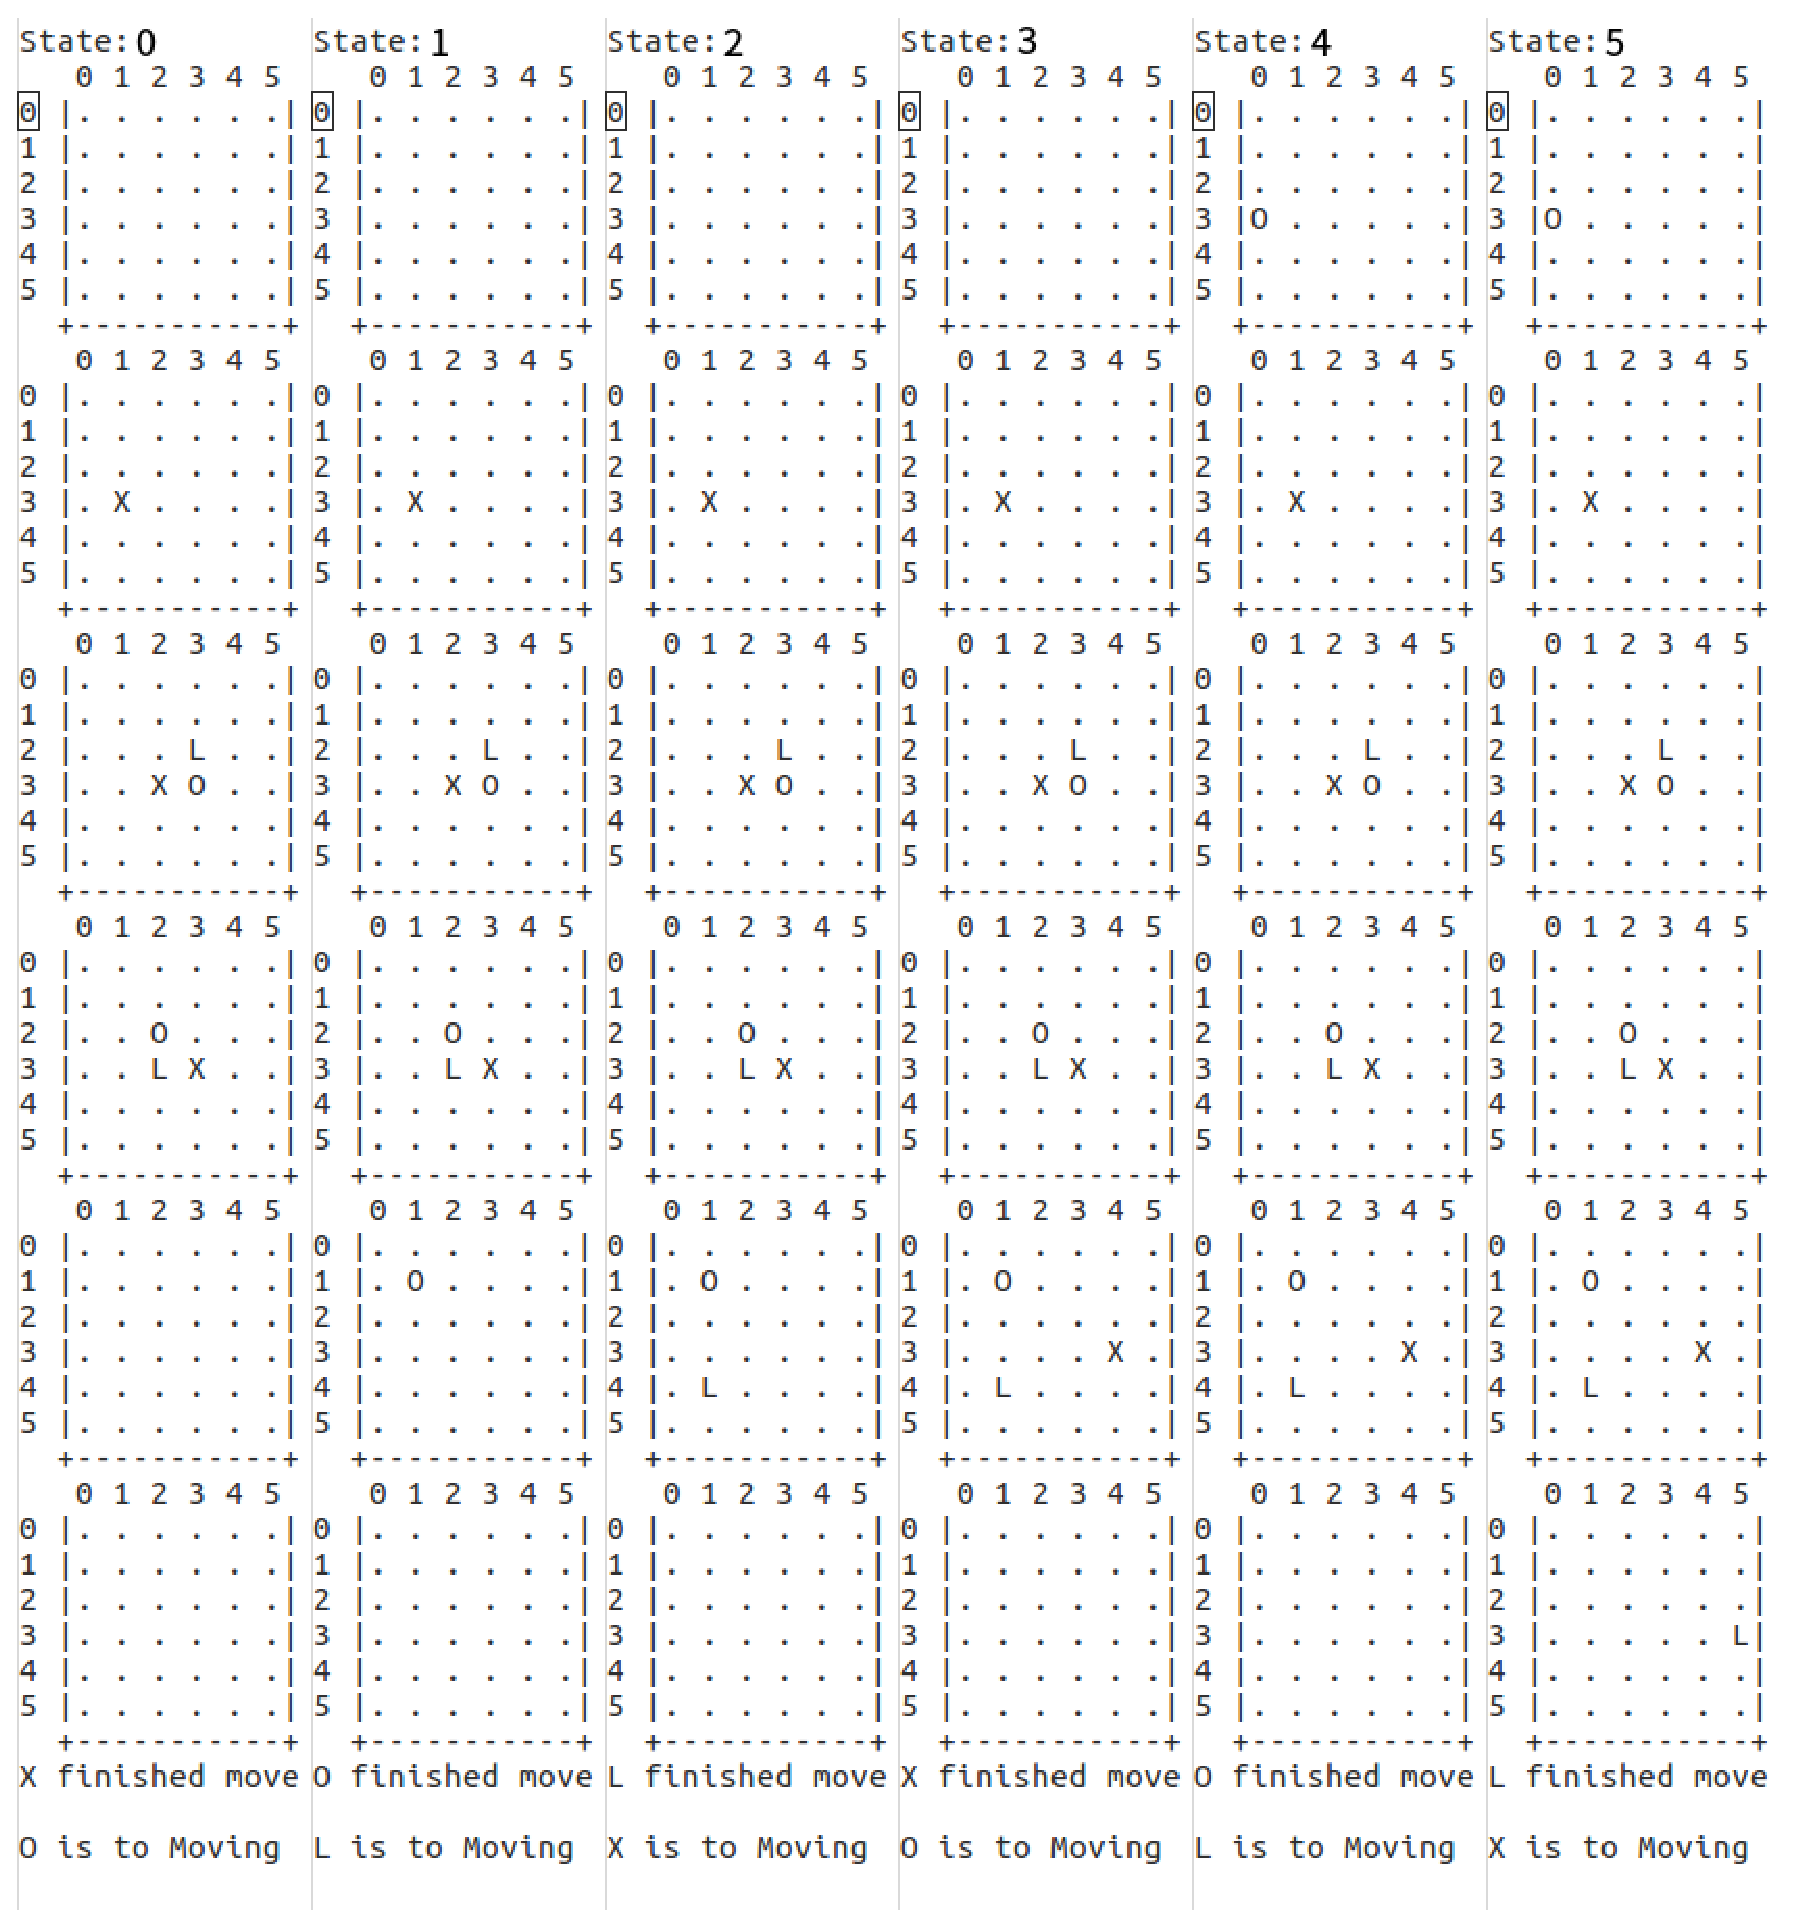
\includegraphics[width=\linewidth]{state.eps}}
	\caption{合理的对战结果}
	\label{result}
\end{figure}	

接下来也尝试了各种改进的组合,具体结果如下
其中,策略分别为
\begin{enumerate}
	\item Selection的Policy改变
	\item 添加合理的剪枝策略
	\item 合并迭代的搜索树
	\item 按照随机次数来衰减模拟结果
\end{enumerate}

而效果就是能否进行合理的比赛,所谓合理的比赛就是指不会出现上述的情况。
因为没有办法很好的度量这个合理性,大致就以一下四个级别:
经常不合理,有时不合理,有时合理,经常合理。(按照多次模拟之后获得实验结果进行统计获得)
\begin{table}[htbp]
	\centering
	\caption{\bf 组合效果分析}
	\begin{tabular}{cc}
		\hline
		组合策略 & 效果  \\
		\hline
		$1,2$ & 有时合理 \\
		$1,3$ & 有时合理 \\
		$2,3$ & 经常合理 \\
		$1,2,3$ & 经常合理 \\
		$1,3,4$ & 经常不合理 \\
		$2,3,4$ & 经常不合理 \\
		\hline
	\end{tabular}
	\label{tab:result1}
\end{table}

同时,由于$1,2,3$组合效果最好,之后,也对该改进MCTS算法和原来的算法进行性能上的分析。按照每下一步所需要的时间和内存来刻画。

相关软硬件状态:
\begin{itemize}
	\item CPU:Intel® Core™ i7-6700K CPU @ 4.00GHz × 8 
	\item Memory:31.4G
	\item OS:Ubuntu 16.04 64bits
\end{itemize}

结果如下:

\begin{table}[htbp]
	\centering
	\caption{\bf 组合效果分析}
	\begin{tabular}{cccc}
		\hline
		策略 & time(s) & virtual(GB) & physics(GB) \\
		\hline
		原生MCTS & 193 & 10.6 & 10.4 \\
		改进MCTS & 245 & 11.1 & 10.8 \\
		\hline
	\end{tabular}
	\label{tab:result2}
\end{table}

当然需要注意的是:这边改进后的程序会保留每一次之前计算落子的结果,但是不用担心,因为当确认落下一子之后,其他无关的状态都会删除掉,所以不会造成内存的快速增长。
\end{adjustwidth}

\subsection{$\cdot$复杂度分析}
\begin{adjustwidth}{2em}{}	
	\ \ \ \ \
	相对而言,这一类启发式类型的算法比较难进行复杂度分析,因为这一类启发式问题主要针对的解决目标就是NP-hard之上的问题,所以进行复杂度分析的意义并不是很大。	
\end{adjustwidth}
\section{结论}
	本文讲MCTS推广到了多人对弈的情况,并通过具体的游戏来进行说明问题。通过一系列方法以一种教优雅的方式解决了原生MCTS推广到多人对弈的问题,能够通过较小的迭代次数来对多人博弈问题进行更优的分析。同时,值得一提的是,以上的改进方法还保持着较好的性能,改进MCTS在各种性能并没有比原生MCTS性能太差。

\section{其他的想法}
由于时间有限,因此还有一些想法并没有付诸实践,然而也一并记录于此。

AlphaGo除了利用MCTS以外,还使用了CNN这类的神经网络,在选择下一步的时候,将两者的进行综合考量。然而实用CNN本身固然很合理,可以将当前局面看做类似与图像,并且具有局部性的考虑。然而个人认为依然可以添加RNN进入到该算法上,更好利用之前的信息,甚至有希望的话,可能能够考虑这一连串步骤背后的意图。


%Manual citation list
\begin{thebibliography}{1}
\bibitem{AlphaGo}
Yuandong Tian, Yan Zhu, \emph{Better Computer Go Player with Neural Network and Long-Term Prediction,} ICLR 2016.
\bibitem{MCTS}
 G.M.J.B. Chaslot, M.H.M. Winands, J.W.H.M. Uiterwijk, H.J. van den Herik; B. Bouzy, \emph{Progressive Strategies for Monte-Carlo Tree Search, } New Mathematics and Natural Computation. 2008
\bibitem{MCTSMPG}
Prof. dr. ir. R.L.M. Peeters, Dr. M.H.M. Winands, \emph{Monte-Carlo Tree Search for Multi-Player Games, } Optima Grafische Communicatie, Rotterdam, The Netherlands. 2013
\bibitem{MCTSGraphWiki} Monte Carlo tree search Graph, wikipedia https://en.wikipedia.org/wiki/Monte\_Carlo\_tree\_search.
\bibitem{MCTSbasecode} https://github.com/PetterS/monte-carlo-tree-search.git
\end{thebibliography}


\end{document}
